%% SECTION HEADER /////////////////////////////////////////////////////////////////////////////////////
\section{Experimental setup for \acl{hsc} model validation}
\label{sec:setup}
%% SECTION CONTENT ////////////////////////////////////////////////////////////////////////////////////
\begin{figure}[!htb]
	\begin{center}
		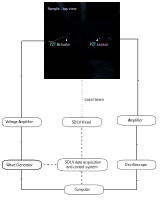
\includegraphics[width=0.95\textwidth]{Chapter_6/setup}
	\end{center}
	\caption{Experimental setup for (1) the \acf{sldv} measurement (dashed line), and (2) the \acf{pzt} wave acquisition (solid line)}
	\label{fig:setup}
\end{figure}
Results from two experimental studies validated the presented model of \ac{hsc}.
The first study was performed for determination of the full wavefield of the propagating waves by the \ac{sldv} (Polytec PSV–400).
The second one was performed for wave acquisition by the \ac{pzt} sensor.
A schematic of the experimental setup is shown in Figure~\ref{fig:setup}.

The \ac{sldv} is method for non-contact measurement of the vibration velocity of structure surface \cite{staszewski2004structural, zak2012damage}.
The principle of vibrometer operation is based on the Doppler effect, recording the change of frequency of the light beam reflected from the vibrating surface.
In laser vibrometry, the measurement of frequency change is realised by interferometer and analysis of both reference and measurement light beam.
The measuring system is additionally equipped with mirrors allowing to change the angle of the measuring beam, so it is possible to take measurements at a grid of points on a surface of inspected structural element automatically.
The \ac{sldv} setup is presented in Figure~\ref{fig:sldv}.
\begin{figure}[!htb]
	\begin{center}
		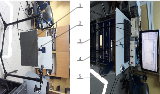
\includegraphics[width=0.95\textwidth]{Chapter_6/sldv}
	\end{center}
	\caption{The \acl{sldv} setup: 1 - the laser sensor head, 2 - the \acl{hsc} specimen, 3 - the arbitrary waveform generator, 4 - the amplifier, 5 - data management system}
	\label{fig:sldv}
\end{figure}

The \ac{pzt} elastic wave generation and acquisition system is used to measure the voltage changes of transducers due to their mechanical deformation.
This is a spot measurement at the location where the sensor has been attached.
A data management unit is responsible for executing prepared tasks and collecting data recorded during measurements.
An arbitrary waveform generator is the source of the low voltage signal, which feeds the Lamb wave detection system and high voltage amplifier.
The amplified signal is intended for the actuator to excite a wave in the sample.
The registered signals by the sensor are amplified by the charge amplifier and supplied to an oscilloscope via a splitter.
The setup used for measurements is shown in Figure~\ref{fig:pzt_setup}.
\begin{figure}[!htb]
	\begin{center}
		\includegraphics[width=0.95\textwidth]{Chapter_6/pzt_setup}
	\end{center}
	\caption{The \acl{pzt} setup, (\textbf{a}) the elastic wave generation and acquisition instruments:  DMU - the data management unit, G1,G2 - the arbitrary wave generator, O - the oscilloscope, HVA - the high voltage amplifier, LWDS - the Lamb Wave Detection Systems, (\textbf{b}) the specimen with the \acfp{pzt}}
	\label{fig:pzt_setup}
\end{figure}

Both methods have some advantages and disadvantages, listed in Table~\ref{tab:method_comp}.
The greatest advantage of the \ac{sldv} technique is the non-contact surface measurements.
If three heads of the laser sensor are available then three-axes of velocity measurements are possible.
However, this method is unsuitable for in-service testing of structures due to its large size and the need to guarantee conditions that prevent signal interference. Therefore, \ac{sldv} is often used in laboratory conditions or when the facility is in maintenance mode.
On the other hand the \ac{pzt} setup is a rather low cost instruments for spot recording of the wave propagation.
The measurements are characterized by high repeatability and can be performed on the construction in operation.

\begin{table}[!htb]
	\small
	\tabcolsep=0.2cm
	%\centering
	\caption{\label{tab:method_comp}Comparison of methods for elastic wave propagation measurements}
	\begin{tabular}{p{0.1\textwidth}>{\raggedright}p{0.4\textwidth}>{\raggedright \arraybackslash}p{0.4\textwidth}}
		\toprule
		\textbf{Method} &\textbf{Advantages} & \textbf{Disadvantages}\\
		\midrule
		\multirow{5}{*}{\ac{sldv}}   & \tabitem automatic full-field scanning & \tabitem high-cost equipment\\ 
		& \tabitem non-contact measurement & \tabitem low signal-to-noise ratio\\
		& \tabitem \ac{3d} velocity vector (optional)& \tabitem special surface treatment is needed, e.g. application of retro-reflective tape\\
		& & \tabitem relatively large space need for measurements \\
		& & \tabitem special sample mounting for repeatability of measurements\\
		\midrule
		\multirow{5}{*}{\ac{pzt}} & \tabitem low-cost instruments & \tabitem spot measurement\\
		& \tabitem high repeatability of measurements & \tabitem displacements vector correlated with the sensor polarization\\
		& \tabitem measurements on the sample in motion & \tabitem cumbersome wiring\\
		& \tabitem generation and recording signals with the same setup & \tabitem sensitive to electric and magnetic fields\\		
		\bottomrule
	\end{tabular}
\end{table}

The specimen comprised of components described in Section~\ref{sec:sample} was fabricated under workshop conditions with rough accuracy.
Before applying the two-ingredient glue (Loctite EA3479B), the bottom surface of the skin was cleaned and degreased with the solvent (Loctite SF7063).
The adhesive curing took 48 hours under a distributed load at ambient temperature.
The top view of the sample is presented in Figure~\ref{fig:sample_dim}.
\begin{figure}[!htb]
	\begin{center}
		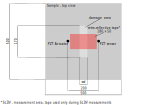
\includegraphics[width=0.95\textwidth]{Chapter_6/sample_dim}
	\end{center}
	\caption{Schematic image of the sample}
	\label{fig:sample_dim}
\end{figure}

The subject of the parametric study was the effect of the disbond size on the propagating \ac{gw}.
A reference measurement of an intact sample was followed by several measurements taken for the subsequent damage introduced on the same specimen.
The damage width varied in range \(\mathrm{w_d}=\left [10, 30, 50, 70, 100, 120 \right ]\) \unit{\mm}, while its fixed length was \(\mathrm{l_d} = 175\) \unit{\mm}.
\nomtypeR[w_dam]{\(w_d\)}{Width of damage}{}{\unit{\metre}}%
\nomtypeR[l_dam]{\(l_d\)}{Length of damage}{}{\unit{\metre}}%
The \(N_c=5\) cycle Hann windowed signal at carrier frequencies \(f_c=[50,100,150]\) \unit{\kHz} was used in the measurements.

The data management unit was used to set measurement parameters, managing them, and saving the collected results.
The arbitrary waveform generator (National Instruments, PXI 1095) generated the low-voltage signal from where it fed Lamb waves detection system (LWDS, Cedrat Technologies) and the actuator (Noliac, NCE51) after 100 times amplification by the  amplifier (Krohn-Hite Corporation, model 7500).
Voltage of the the sensor (Noliac, NCE51) was measured by the oscilloscope (National Instruments, PXI 1095) through the LWDS.
Each measurement was conducted at the temperature of 20\unit{\degreeCelsius} controlled in the environmental chamber (Angelantoni Test Technologies, DM 600C) and averaged 20~times to improve the signal-to-noise ratio.